\section{Descriptive Statistics}\label{Sec:Des_Stat}

Descriptive statistics is an important part of data analysis. Many contexts can be represented by simple graphs and tables. In addition, the descriptive statistics provide a good visualization of the data, as an ancient Chinese proverb says; one picture is worth a thousand words. In this chapter, we will focus on how to build tables and graphs with predefined settings using our own functions. Functions that we have built in this section can be used through customizations by others and is easy to replicate. In the following section the code of 3 quantlets is described and discussed.

\subsection{Implementatition}

In this section we want to show some implementation of R to build tables and graphs. Moreover we focus on variables which are economically important for the regression analysis. The first glance is on the age distribution of the population and the possibly prevailing differences in gender. An appropriate graph for visualizing age distribution is the population pyramid. To plot population pyramid in R, we use the \texttt{plotrix} package, which must be installed before.
\lstset{firstnumber = 157}
\begin{lstlisting}
install.packages("plotrix")
library("plotrix")
\end{lstlisting}
In order to use the plot function \texttt{pyramid.plot} from the \texttt{plotrix}-package we have to calculate the relative frequencies of age distribution according to the gender. Therefore we constructed a function \texttt{frequency}.
\lstset{firstnumber = 161}
\begin{lstlisting}
frequency = function(k, l){
  100*sweep(table(k,l), 2, colSums(table(k,l)), "/")
}
\end{lstlisting}
Function \texttt{frequency} calculates a table with frequencies of the variable k with different characteristics which are given in l. In our case we determine k as the age variable \texttt{dat\$ef41} and l as gender \texttt{dat\$ef10}. Function \texttt{frequency} uses sweep function and relies on summary statistics such as colSum for calculating relative frequancies of different age of male and female subjects, this results in following table:
\begin{table}[h!]
\centering
\caption{Frequency table generated by the function \texttt{frequency(dat\$ef41, dat\$ef10)}}
\label{freq}
\begin{tabular}{l|c|c|}
\cline{2-3}
                                 & \multicolumn{2}{c|}{\textbf{l}} \\ \hline
\multicolumn{1}{|l|}{\textbf{k}} & männlich       & weiblich       \\ \hline
\multicolumn{1}{|l|}{16}         & 0.2446         & 0.1777         \\ \hline
\multicolumn{1}{|l|}{17}         & 0.5249         & 0.4334         \\ \hline
\multicolumn{1}{|l|}{18}         & 0.8379         & 0.7812         \\ \hline
\multicolumn{1}{|l|}{...}        & ...            & ...            \\ \hline
\multicolumn{1}{|l|}{66}         & 1.2839         & 0.8838         \\ \hline
\end{tabular}
\end{table}

The function \texttt{buildpopulation} was generated to produce and simultaneously save the population pyramid graphic in a separate pdf file. Such functions are very useful especially if you want to create a lot of similar plots, which should always have the settings to look uniform. However, such settings can be permanently defined in the function or can also be defined as a freely selectable variable.
\lstset{firstnumber = 170}
\begin{lstlisting}
buildpopulation = function(k, l, popname){
  pop = frequency(k, l)
  pdf(popname)
  	pyramid.plot(pop[,1], pop[,2], labels = rownames(pop), gap = 2, lxcol = "blue", rxcol = "red")
  dev.off()
}
\end{lstlisting}
The function \texttt{buildpopulation} uses variables k and l which are neccessary for the \texttt{frequency} function and popname for setting a name for the graphic such as \glqq populationpyramid.pdf\grqq{}. Within the function \texttt{buildpopulation} the results of the \texttt{frequency} function are assigned to an auxiliary variable pop. This merely serves for a better overview in the further use of the generated results of the \texttt{frequency} function in the \texttt{pyramid.plot} and is not absolutely necessary. Since we are interested in union wage effects, we therefore investigate the age distribution of the union covered population and a population without any union contract. Therefore we generate a subsample with a data which include only union covered workers such as:
\lstset{firstnumber = 183}
\begin{lstlisting}
datFCSC = dat[ which(FC == 1 | SC == 1),]
\end{lstlisting}
Starting from the subsample we can finally build the population pyramid using the function \texttt{buildpopulation}. The same approach is used for the population pyramid for workers without a union contract. Defining such subsample we have to ensure that the worker neither covered by on sectoral collective nor firm contract (\texttt{.which(FC == 1 | SC == 1)}). 
\lstset{firstnumber = 189}
\begin{lstlisting}
buildpopulation(datFCSC$ef41, datFCSC$ef10, "populationFCSC.pdf")
\end{lstlisting}
This results in the following two graphics: 

\begin{minipage}[t]{0.475\textwidth}
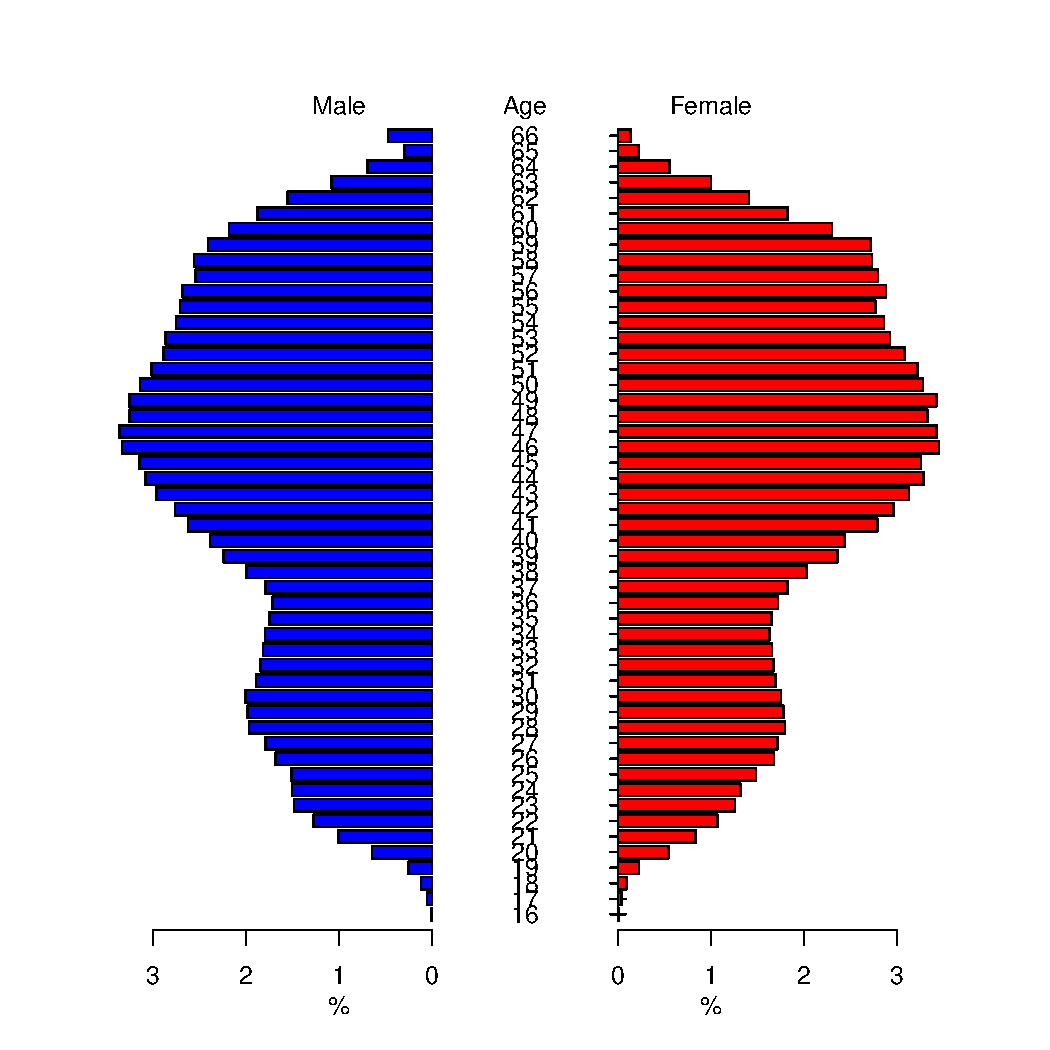
\includegraphics[width=\textwidth]{populationFCSC}
\captionof{figure}{Population pyramid of employees covered by a union contract}
\label{fig:popFCSC}
\end{minipage}
%\hfill
\begin{minipage}[t]{0.475\textwidth}
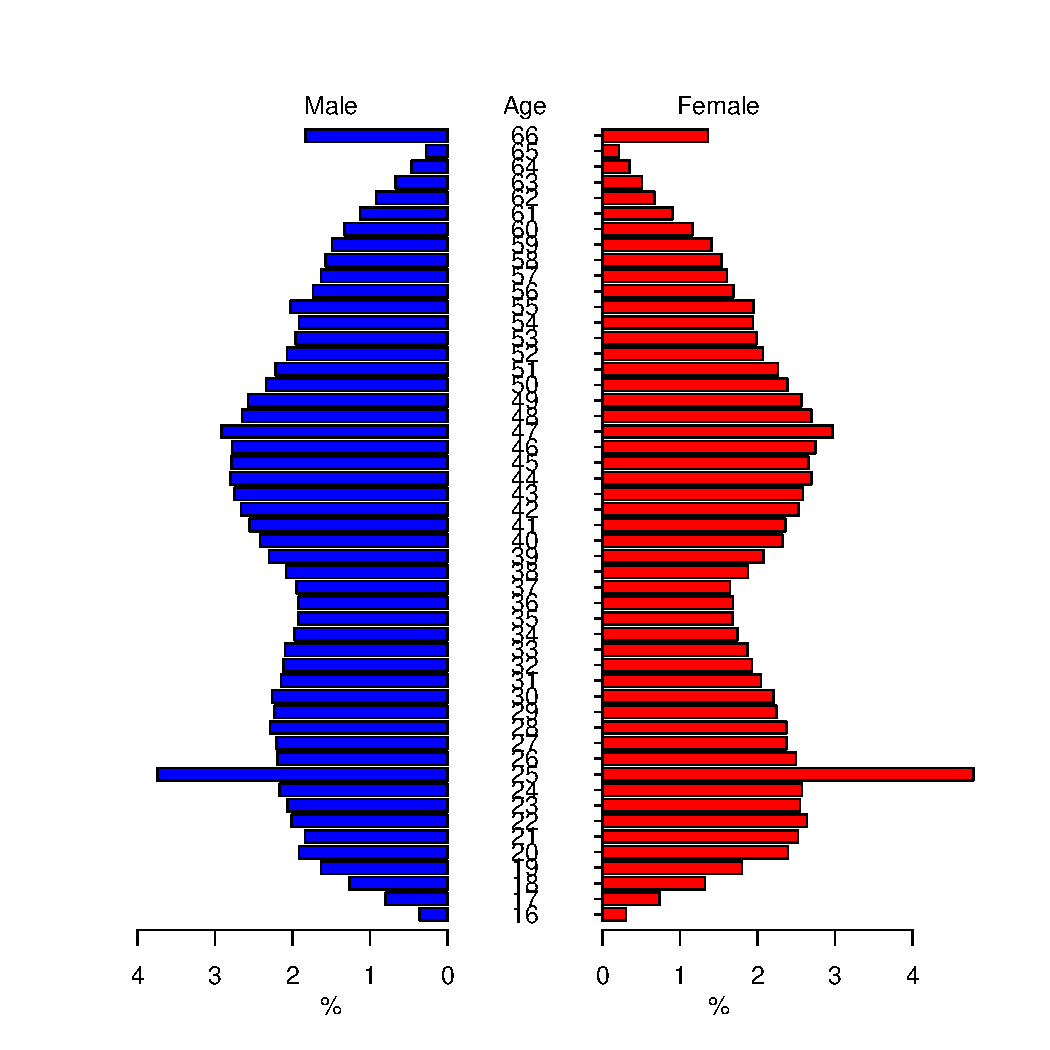
\includegraphics[width=\textwidth]{populationNoFCSC}
\captionof{figure}{Population pyramid of employees not covered by a union contract}
\label{fig:popNoFCSC}
\end{minipage}
\vspace{0.5cm}


Due to the visualisation of the data by the population pyramid, there are no recognizable differences in the age structure between man and woman in both subsamples. However, the general age distribution in the group of workers with a union contract differs from the workers without. Population with a union contract seems to be older than the population without. To fix this statement numerically, we calculate the median. Indeed the average age of the workers with a trade union contract is 45 years, while the average age of the workers without a union contract is 40.

The function \texttt{buildboxplot} was created following a similar principle to the function \texttt{buildpopulation}, which generates and saves the graphic in a pdf file.
\lstset{firstnumber = 208}
\begin{lstlisting}
buildboxplot =  function (v, w, boxname, z){
  pdf(boxname, width = 11, height = 7)
  boxplot(v~w, range=2.5, width=NULL, notch=FALSE,varwidth=FALSE, names = z,
          boxwex=0.8, outline=FALSE, staplewex=0.5, horizontal=FALSE, border="black",
          col="#94d639", add=FALSE, at=NULL)
  abline(h = median(v, na.rm = TRUE), col = "red")
  dev.off()
}
\end{lstlisting}

Function \texttt{buildboxplot} uses four characteristics: v, w, boxname and z. V is a numeric variable and w is a group variable into which the numeric variable v will be splitted. Using boxname we can predetermine the name of the file such as \glqq boxplot\_ lnwage\_ education.pdf\grqq{}. Z is a vector with label names of the group variable w, so that the length of the vector z agrees with the number of the levels in w. Within the \texttt{buildboxplot} function we insert into the boxplot a red line which characterises the median of the numeric variable v in the investigated population.
\lstset{firstnumber = 240}
\begin{lstlisting}
buildboxplot(data$lnwage, data$ef16u2, "boxplot_lnwage_education.pdf", educLAB)
\end{lstlisting}
The results of the \texttt{buildboxplot} function are shown in the figure \ref{Fig:boxplot}.
\begin{figure}
\begin{center}
\caption{Boxplot of education differences in ln(Wage)}
\label{Fig:boxplot}
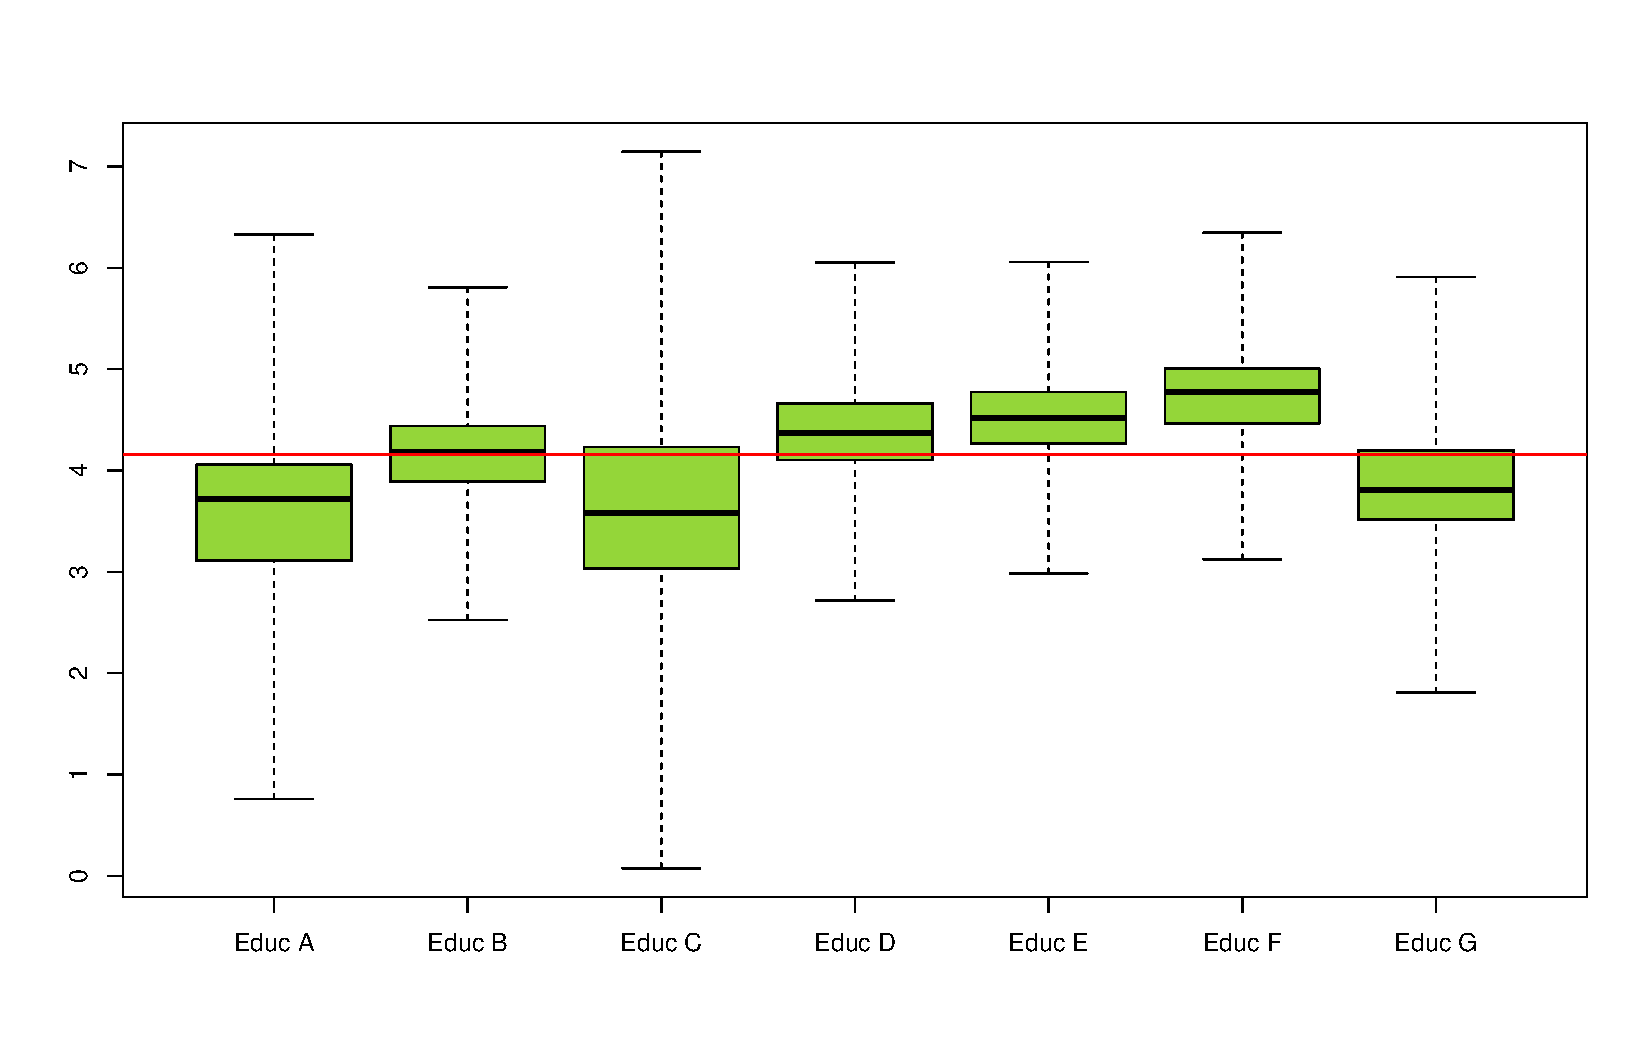
\includegraphics[scale=0.55]{boxplot_lnwage_educ}
\end{center}
\end{figure}
The figure \ref{Fig:boxplot} shows ln(Wage) distribution over different education levels. Education level \texttt{educLab} results following characteristics:
\begin{itemize}
\setlength\itemsep{0em}
\item \textbf{Educ A:} Middle school without vocational training;
\item \textbf{Educ B:} Middle school with vocational training;
\item \textbf{Educ C:} High school without vocational training;
\item \textbf{Educ D:} High school with vocational training;
\item \textbf{Educ E:} Professional university degree;
\item \textbf{Educ F:} University degree;
\item \textbf{Educ G:} Education unknown.
\end{itemize}
The higher the level of education of the worker the higher the median wage in this education group. This is in line with the basic theory of human capital. A middle school and high school education leads to higher wages when a vocational training has been completed afterwards (compare groups Educ A and C with Educ B and D). By using the subsamples, we can again create two graphs with workers with union contract and workers without.\footnote{Please see appendix B Figures \ref{Fig:educFCSC} and \ref{Fig:educNoFCSC} for a comparison of the wages distribution over different education level in different subsamples.} The workers with union contract earn on average more than those without. But also the wage distribution in the same education group differs strongly in the subsamples. While the wage distribution in the subsample with union contract is more homogenous, there is a large variation in the subsample with workers without a union contract especially in groups with a lower education level.

In this part we will present the functions used in our quantlet 4. Functions \texttt{quant} and \texttt{buildquantileplot} are made to examine correlations between two numeric variables along the quantiles e.g. the effect of work experience along the wage distribution. First we build a function \texttt{quant(x,y,q)} for calculating quantiles. Along the variable x the function calculates for every $x_{i}$ a quantile q of the variable y. The vector q consists of the quantiles we want to investigate and can be changed as desired. The vector color must have the same number of elements as the vector q, since each q is assigned a color.
\lstset{firstnumber = 255}
\begin{lstlisting}
  quant = function(x,y,q){
                  aggregate(x, y, na.rm=TRUE, quantile, q)
  }

  q = c(0.10, 0.25, 0.50, 0.75, 0.90)
  color = c("orange", "red", "green", "blue", "black")
\end{lstlisting}
Using the quantiles which are aggregated by the function \texttt{quant}, we can build a scatterplot with the quantile lines. Therefore we build a function \texttt{buildquantileplot} which contains a simple scatterplot of the independent variable x and dependent variable y. Using \texttt{xla} and \texttt{yla} we can add labels to a plot and using \texttt{plotname} determine the name of the pdf file. Such scatterplot can be applied to any problems where the quantile distribution maybe different. It is  useful graph to have a look to quantile distribution of a numeric variable and could be helpful to state an appropriate regression method.
\lstset{firstnumber = 277}
\begin{lstlisting}
buildquantileplot = function(x, y, xla, yla, plotname){
  pdf(plotname)
  #plot points
  plot(x, y, ylim=c(2,8), pch = 1, col='dark green',
       xlab = xla, ylab = yla)
  #plot quantilelines
  for (l in 1:length(q)){
    lines(quant(y, list(x), q[l]), col = color[l], lwd =2)
  }
  dev.off()
}
\end{lstlisting}
Using the \texttt{for loop}, we add the quantile lines to the scatterplot, the quantiles already defined in q.
\lstset{firstnumber = 303}
\begin{lstlisting}
buildquantileplot(datNoFCSC$ef40, datNoFCSC$lnwage, "Experience", "Ln(wage)",
		  "scatterplot_lnwage_experience_NoFCSC.pdf")
\end{lstlisting}
After executing the function \texttt{buildquantileplot} with the dependent variable ln(wage) (\texttt{dat\$lnWage}) and independent variable experience (\texttt{dat\$ef40}). The following graph demonstrates relation between the wages and work experiances along different wage quantiles, which we will analyse in more detail below using the quantile regression.
\begin{figure}
\begin{center}
\caption{Effect of work experiences along the wage distribution}
\label{Fig:scatter}
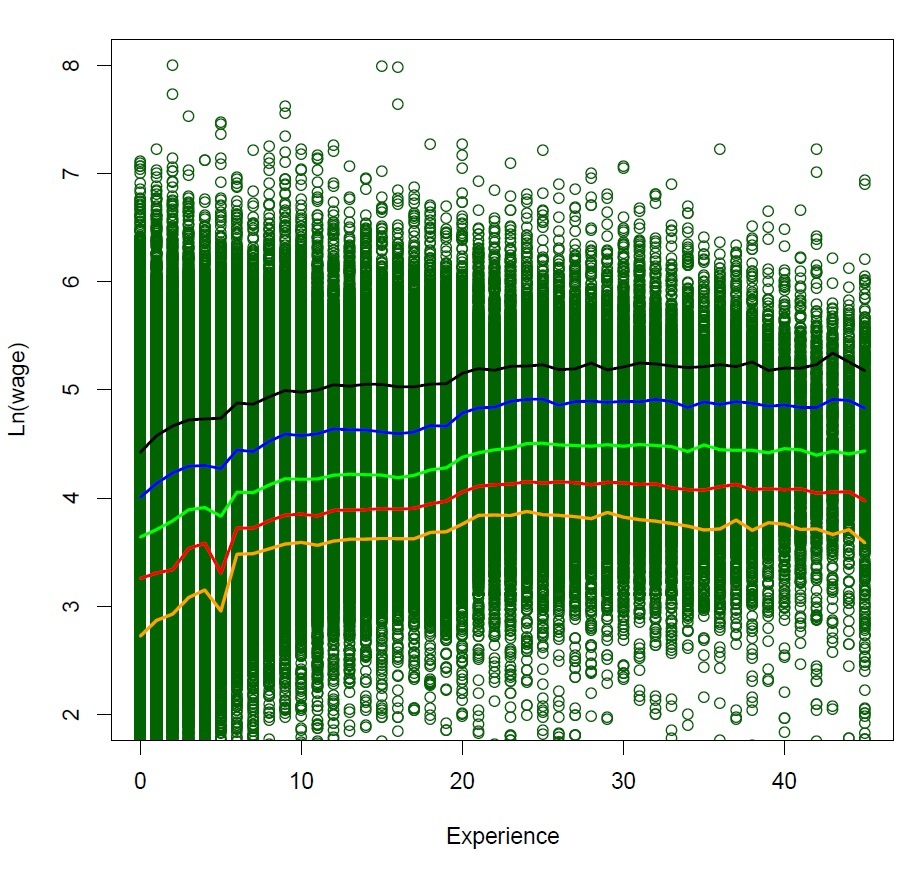
\includegraphics[scale=0.4]{scatterplotNoFCSC-lnwage-experience}
\end{center}
\end{figure}
The quantile lines in the scatterplot of the subsample with the workers without a union contract have all the same positive trend but different slopes. Therefore the quantile regression seems to be more appropriate than the ordinary least square approach. Nevertheless, this statement is subjective and will be examined in the section \ref{Sec:Regression}.

We distinguish between three different union bargaining regimes:\\
\noindent\hspace*{6mm} (SC) refers to a sectoral collective contract, which is negotiated between employer's associations and employee unions,\\
\noindent\hspace*{6mm} (FC) refers to a firm contract, which is negotiated between an employee's union and a single firm, and\\
\noindent\hspace*{6mm} (IC) refers to contracts, individually negotiated between employee and employer. And we extend the econometric analysis to female employees in order to be able to make statements regarding the gender wage gap at mean wages and across quantiles. The challenge of the following part namely our quantlet 5 is to create a table with the information stated above. Such a table shall contain the mean and the standard deviation  of the hourly log wages and the share of different union contracts.
Since those calculations in a data frame are time-consuming in case of large data, we convert first the data frame into a data table. Therefore we install  neccessary package and put it into our local \texttt{R} library:
\lstset{firstnumber = 319} 
\begin{lstlisting}
dat = data.table(dat)             
\end{lstlisting}
The variable \texttt{Group} is created by using the three dummy variables which are labled in \texttt{Group} as 1: SC , 2: FC and 3: IC. Excluding all \texttt{NA}'s we generate the number of observations according to the new variable \texttt{Group}, which is neccessary for further calculation of the $\log$ mean wage and the standard deviation for each group and each gender.
\lstset{firstnumber = 330} 
\begin{lstlisting}
sum = dat[!is.na(Group), .N]                                 
\end{lstlisting}
Following code shows how to order the results by gender:
\lstset{firstnumber = 333} 
\begin{lstlisting}
lnWageSummary = dat[!is.na(Group), .(LogHourlyWageMean = mean(lnWage, na.rm = T),         
                                     LogHourlyWageSD = sd(lnWage, na.rm = T)), by = .(ef10, Group)]  
lnWageSummary = lnWageSummary[order(ef10, Group)]                                   
\end{lstlisting}
Exactly the same procedure will be done for overall population. Using the \texttt{table} function we generate the absolute frequencies of SC, FC and IC devided by gender.
\lstset{firstnumber = 347} 
\begin{lstlisting}
mtable = table(dat$Group, dat$ef10)                                            
\end{lstlisting}
The same approach is applied to construct employee share and order it by \texttt{Group}. The already existing results are packed into a table in the following step where we use the \texttt{prop.table} function to provide the proportion of the employees of different level of the variable \texttt{Group} and for female and male subjects:
\lstset{firstnumber = 356} 
\begin{lstlisting}
lnWageSummaryTotal = data.frame(Regime       = c("SC", "FC", "IC"),                                   
                     MaleEmpolyeeShare       = prop.table(mtable, 2)[, 1],  
                     MaleLogHourlyWageMean   = lnWageSummary[ef10 == "maennlich", LogHourlyWageMean],    
                     MaleLogHourlyWageSD     = lnWageSummary[ef10 == "maennlich", LogHourlyWageSD],       
                     FemaleEmpolyeeShare     = prop.table(mtable, 2)[, 2],                             
                     FemaleLogHourlyWageMean = lnWageSummary[ef10 == "weiblich", LogHourlyWageMean],                            FemaleLogHourlyWageSD   = lnWageSummary[ef10 == "weiblich", LogHourlyWageSD],     
                     TotalEmpolyeeShare      = TotalEmpolyeeShare$Share,                                                        TotalLogHourlyWageMean  = lnWageSummaryOverall$LogHourlyWageMean,                
                     TotalLogHourlyWageSD    = lnWageSummaryOverall$LogHourlyWageSD,                                            stringsAsFactors        = FALSE)                                          
\end{lstlisting}
The calculation and creation of the row \texttt{total} is similar to the first part and not further commented in the quantlet 5. Created vector \texttt{total} is added to the data frame \texttt{lnWageSummaryTotal}. Few corrections using some basic R functions can make the output much more readable. Using function \texttt{rapply} we transform all numbers into a numeric value and round the results by setting \texttt{digit} to 2.
\lstset{firstnumber = 401} 
\begin{lstlisting}
lnWageSummaryTotal[,2:10] = rapply(lnWageSummaryTotal[,2:10], as.numeric)
lnWageSummaryTotal        = rapply(object = lnWageSummaryTotal, f = round, classes = "numeric", how =       "replace", digits = 2)
\end{lstlisting}
At the end of the quantlet the data which was temporary stored in the data table format is transformed back into a data frame. R provides a very useful package \texttt{xtable}, which makes it possible to print the table in a tex-file. This is a great advantage of R compared to other software. It allows the scientist to transfer the results smoothly into the report paper. Above all, it is useful and requires little effort if the data change. 
\lstset{firstnumber = 405} 
\begin{lstlisting}
dat = data.frame(dat)   
install.packages("xtable")
library(xtable)
print(xtable(lnWageSummaryTotal, type = "latex"), file = "covRegimeandLNWages.tex")
\end{lstlisting}

Table \ref{Coverage Regime} summarizes the shares of coverage regime affiliations as well as mean log wages for male and female employees under the different bargaining regimes in the GSES 2010 sample. $33\%$ of male employees ($37\%$ of female employees) are covered by a sectoral contract and $6\%$ of both male and female employees are covered by contracts negotiated on the firm-level. These figures are lower than the coverage ratios obtained by \cite{Fitzenberger&Kohn&Lembcke:13} in their analysis of the 2001 data. The literature confirms, that this is due to a decline in collective coverage in recent years \citep{Addison&Bryson&Teixeira&Pahnke6Bellmann:13}. A possible explanation for the discrepancy is that the sample of employees is not representative for the population. The proportion of employees in the sample from large firms compared to all employees in large firms is lower than the proportion of employees from smaller firms.
\begin{table}[h]
\scriptsize
\centering
\caption{Coverage Regime Affiliation and Log Wages for Male and Female Employees}
\label{Coverage Regime}
\begin{tabular}{l|ccccccccccc}
\multicolumn{4}{c}{male}                                                                               & \multicolumn{3}{c}{female}             &\multicolumn{3}{c}{overall}                                                              \\
\hline
\multirow{2}{*}{regime} & \multirow{2}{*}{employee-share} & \multicolumn{2}{l}{log hourly wages}    & \multirow{2}{*}{employee-share} & \multicolumn{2}{l}{log hourly wages}    & \multirow{2}{*}{employee-share} & \multicolumn{2}{l}{log hourly wages}\\
                        &                       & mean    & std. dev.   &                                         & mean           & std. dev.         &                   & mean           & std. dev.          \\
\hline
SC                      &     $0.33$     &   $4.34$     &   $0.47$   &                       $0.37$           &   $4.24$     &   $0.41$                             &$0.35$&$4.29$& $0.44$\\
FC                      &     $0.06$     &   $4.41$     &   $0.41$   &                       $0.06$           &   $4.24$     &   $0.34$                             &$0.06$& $4.33$& $0.39$\\
IC                      &     $0.61$     &   $4.08$     &   $0.73$   &                       $0.57$           &   $3.81$     &   $0.61$                             &$0.59$& $3.97$& $0.69$\\
total                   &     $1.000$     &   $4.19$     &   $0.65$   &                       $1.00$           &   $4.01$     &   $0.56$                            &$1.00$& $4.11$& $0.62$\\
\hline
\end{tabular}
\end{table}
Mean log hourly wages are highest among employees with firm-specific collective contracts. Employees under firm-specific coverage earn more on average than employees having individually negotiated their contract, suggesting that there is a union wage premium. Moreover, women earn less than men regardless of the coverage regime. Concluding from the standard deviation figures, wage dispersion is highest among employees, not covered by a collective agreement and higher among male employees.

\subsection{Testing}

The section \ref{Sec:Des_Stat} consists of 3 quantlets and 5 own functions. In order to use the functions correctly by others, following control command is implemented in each function:
\lstset{firstnumber = 162} 
\begin{lstlisting}
  if (missing(k))
    stop("No data passed to the function. Variable k has to be determined.")
\end{lstlisting}
In the first line we check if the variable necessary for the execution of the function is missing. If it is missing, an error message is displayed stating that a variable must still be determined to execute the function. We have installed this error message in each of our functions for each variable.

In the second part of the error messages the numeric variables are checked explicitly. We can explain this by the examples of the functions \texttt{frequency} and \texttt{quant}. The function \texttt{frequency (k, l)} uses the variable k and l, in which case no variable must necessarily be a numerical variable since only the relative frequencies are calculated. Let's look at a concrete example: \texttt{frequency(dat$ef16u2, dat$ef10)}. We execute the function \texttt{frequency()} with two non numeric variables: education and gender. Indeed our function calculates the relative frequencies. Note that the sum over the one column is 100\%. If we want to check in advance whether a variable is numeric, we execute the command \texttt{is.numeric()}. If the variable is numeric then we get the value \texttt{TRUE} otherwise \texttt{FALSE}. The function \texttt{quant(y, x, q)} again uses three variable and two of them must be numeric. This applies to the variables \texttt{y} and \texttt{q}. Variable \texttt{q} defines the quantile to be calculated, which can be either a number like \texttt{q = 0.5} (also called median) or a vector \texttt{q = c (0.25, 0.5, 0.75)}. Variable y must be numeric because the quantile is calculated for this variable. For this reason, the following error messages are installed in the function quant:
\lstset{firstnumber = 262} 
\begin{lstlisting}
  if (is.numeric(y) != TRUE)
    stop("Numeric data needed. y has to be numeric")
  if (is.numeric(q) != TRUE)
    stop("Numeric data needed. Quantile q was wrong specified.
    q can be either a number or a numeric vector.")
\end{lstlisting}

Our \texttt{buildpopulation} and \texttt{buildquantileplot} functions call up other functions such as \texttt{quant} and \texttt{frequency}, so the error messages which were already executed in the implemented \texttt{quant} and \texttt{frequency} functions are no longer implemented in the new code of the function e.g. \texttt{buildpopulation} to avoid redundancy.

Furthermore in functions \texttt{buildpopulation}, \texttt{buildboxplot} and \texttt{buildquantileplot}, the name of the pdf file is defined in the function header. At the end of the name of the file \texttt{.pdf} must be attached, the entire expression must be specified in quotation marks, and only then plots are built correctly and stored in an external pdf file. If the name is not entered correctly, an error message from R will appear automatically. For example, lets call the function \texttt{buildpoulation(dat\$ef41, dat\$ef10, \"populationFCSC.pdf\")}. This is the correct execution of the function. Let's delete the quotes: \texttt{buildpoulation (dat$ef41, dat$ef10, populationFCSC.pdf)}. Then following error message appears:\\ \texttt{\textcolor{red}{Error in gsub(\dq \%\textbackslash \%\dq , \dq \dq , s) : object \dq populationFCSC.pdf\dq not found}}.\\This means that the pdf file cannot be created because the entered name does not have the correct syntax. Since this error message is already a component in R, it is not possible for us to modify it and to adapt it specifically to our example.
% 
The code of quantlet 5 cannot be really tested as it is specific for our given problem how to calculate the wanted table. One can test the result by using a calculator which would take rather long as we have over $1.5$ million observations or when you work in a team another person can calculate the same table in a different way and compare the results at the end. As we calculated only mean, standard deviation and the shares there are not many sources for errors because those values are almost all calculated by internal functions. Errors could occur from wrongly selected columns in the data table. But these errors are often easy to identify.


\subsection{Conclusion}

The functions of the quantlets created for the descriptive statistic are efficient and can be easily applied to other issues. The functions fulfill their purpose and make the code much more compact and clear. Especially the function quant can show us differences in median and quantiles between groups, which is very useful when comparing groups and when choosing variables for regression.\footnote{ Example: When calling \texttt{quant(dat\$ef41, dat\$ef9, 0.5)}, we can immediately calculate the medians of the variable ages in the different employee groups.} An advantage of construction table \ref{Coverage Regime} is that the calculation is done easily and fast. By using the \texttt{data.table} package the calculation is even faster because the package can handle big data sets easily. Some disadvantages are if you want to export your table into a \texttt{.tex} file you are not as flexible in the layout as when you are doing it just in latex.

